\subsection{Алгоритм Z-буфера}

Алгоритм Z-буфера используется для растеризации поверхностей объектов. Поскольку под поверхностью в рамках этой работы подразумевается часть плоскости, ограниченная некоторым многоугольником, задача растеризации многоугольника и внесения его в буфер сводится к определению принадлежности точки этому многоугольнику и поиску значения координаты $z$ этой точки.

Поскольку плоскость можно задать тремя точками, достаточно взять любые три точки из многоугольника, которым задаётся поверхность объекта. Сделать это можно следующим образом:

Пусть заданы точки $A, B, C$, задающие плоскость в пространстве камеры. $$ \vec{N} = \vec{AB} \times \vec{AC} $$
Теперь, можно записать уравнение плоскости в виде
$$ N_x(x-x_a) + N_y(y-y_a) + N_z(z-z_a) = 0 $$
Раскрыв скобки, можно перейти к следующему виду:
\begin{equation}
    N_xx + N_yy + N_zz - (N_xx_a + N_yy_a + N_zz_a) = 0
    \label{eq:plane}
\end{equation}

Поскольку занесение координат в z-буфер можно производить построчно (последовательно для каждой строки буфера), вычисление координаты z можно производить пошаговым способом (в пределах одной строки)~\cite{Rogers}.

Поскольку в пределах одной строки, $y = const$, глубина пикселя данной строки с координатой $x_1 = x + \Delta x$ можно вычислить по формуле~\ref{eq:z-next}.

\begin{equation}
    z_1 = z - \frac{ a}{ c}
    \label{eq:z-next}
\end{equation}
Где $a$ и $c$ --- коэффициенты уравнения плоскости при $x$ и $z$ из уравнения~\ref{eq:plane}

Для первой точки на каждой из строк, значение координаты $z$ придётся вычислять из уравнения плоскости.

Для определения точек, принадлежащих многоугольникам, можно использовать алгоритмы растровой развёртки многоугольников.

На рисунке~\ref{fig:z-buffer} изображён алгоритм Z-буфера.

\begin{figure}[h!]
    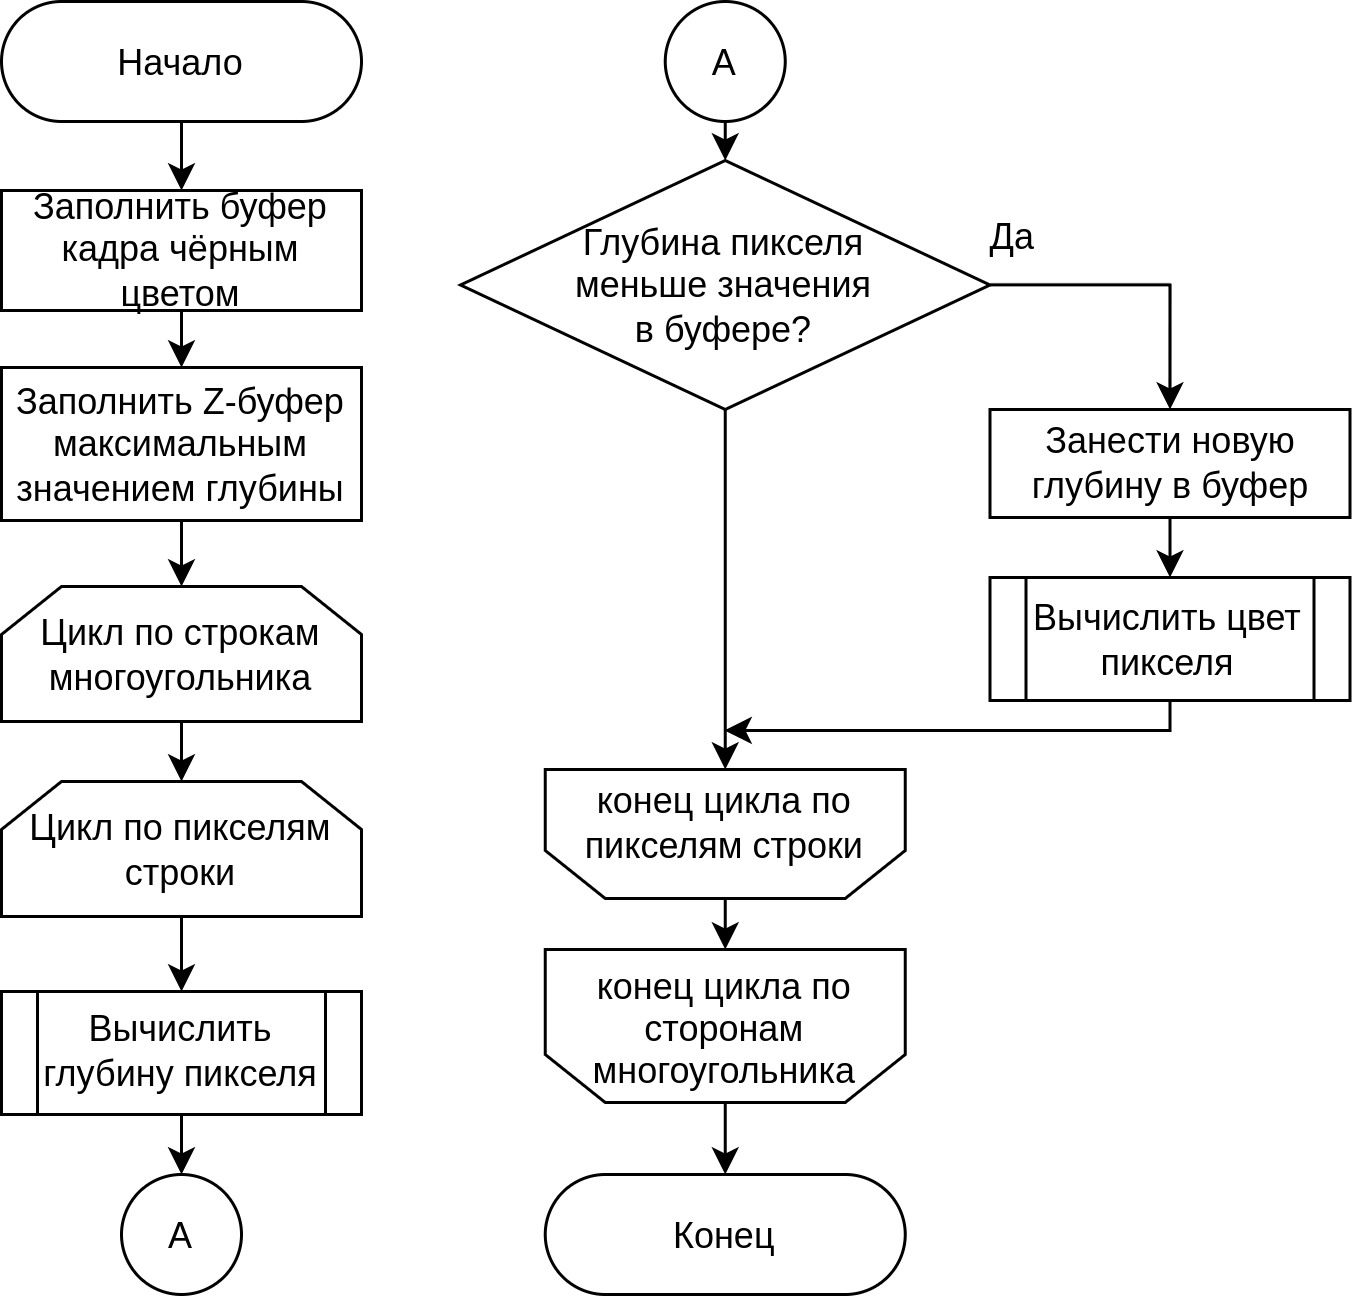
\includegraphics[width=\textwidth]{zbuf.drawio.png}
    \caption{Алгоритм z-буфера для многоугольника}
    \label{fig:z-buffer}
\end{figure}